\documentclass[conference]{IEEEtran}
\IEEEoverridecommandlockouts

\usepackage[utf8]{inputenc}
\usepackage[T2A]{fontenc}
\usepackage[russian]{babel}

\usepackage{cite}
\usepackage{amsmath,amssymb,amsfonts}
\usepackage{algorithmic}
\usepackage{graphicx}
\usepackage{textcomp}
\usepackage{xcolor}

\def\BibTeX{{\rm B\kern-.05em{\sc i\kern-.025em b}\kern-.08em
    T\kern-.1667em\lower.7ex\hbox{E}\kern-.125emX}}


\usepackage{booktabs}
\usepackage{array}
\usepackage{tabularx}
\usepackage{longtable}
\usepackage{multirow}
\usepackage{hyperref}
\usepackage{microtype}
\usepackage{caption}
\definecolor{darkred}{rgb}{0.7,0.12,0.12}
\definecolor{darkgreen}{rgb}{0.08,0.47,0.16}

\begin{document}

\title{Beyond Gaussian Noise: Convergence of Stochastic Optimizers under Correlated and Heavy-Tailed Financial Noise}

\author{%
\IEEEauthorblockN{Дмитрий\,Кортунов}
\IEEEauthorblockA{\textit{НИУ ВШЭ}\\
Москва, Россия\\
dvkortunov@edu.hse.ru}\\
\and
\IEEEauthorblockN{Вадим\,Пастушенко}
\IEEEauthorblockA{\textit{НИУ ВШЭ}\\
Москва, Россия\\
vapastushenko@edu.hse.ru}
\and
\IEEEauthorblockN{Алексей\,Дубовицкий}
\IEEEauthorblockA{\textit{НИУ ВШЭ}\\
Москва, Россия\\
andubovitskiy@edu.hse.ru}
\and
\IEEEauthorblockN{Андрей\,Шадрин}
\IEEEauthorblockA{\textit{НИУ ВШЭ}\\
Москва, Россия\\
arshadrin@edu.hse.ru}
}

\maketitle

\begin{abstract}
Финансовые временные ряды содержат шум различной природы: гауссов,
тяжёлохвостовый, коррелированный и их комбинации. Мы рассматриваем
шумоподавление~--- скользящее среднее, фильтр Калмана, вейвлет-пороговую
обработку, медианный фильтр~--- как этап предобработки и эмпирически
измеряем влияние выбора фильтра на сходимость SGD, Adam и AdamW. Полный
факторный эксперимент $5\times4\times3$ на двух синтетических задачах
(квадратичная, логистическая регрессия) и параллельный эксперимент на
реальных финансовых рядах вскрывает существенный, ранее не
подчёркивавшийся эффект: фильтрация буфера градиентов смещает «сигнальную»
составляющую градиента и в чисто гауссовом режиме на квадратичной задаче
замедляет сходимость; однако в режиме тяжёлохвостового шума медианный
фильтр обеспечивает на 17~дБ больший прирост SNR, чем линейные фильтры, и
стабилизирует сходимость SGD/Adam там, где F0 не сходится. На реальных
дневных лог-доходностях прогностический MSE ухудшается при любом фильтре
(в данных нет «гладкого сигнала»); тем не менее фильтры заметно меняют
структурные характеристики (Хёрст, индекс хвоста), что важно для
согласования с предположениями теории сходимости.

% ════════════════════════════════════════════════════════════════════
\end{abstract}

\begin{figure*}[htbp]
  \centering
  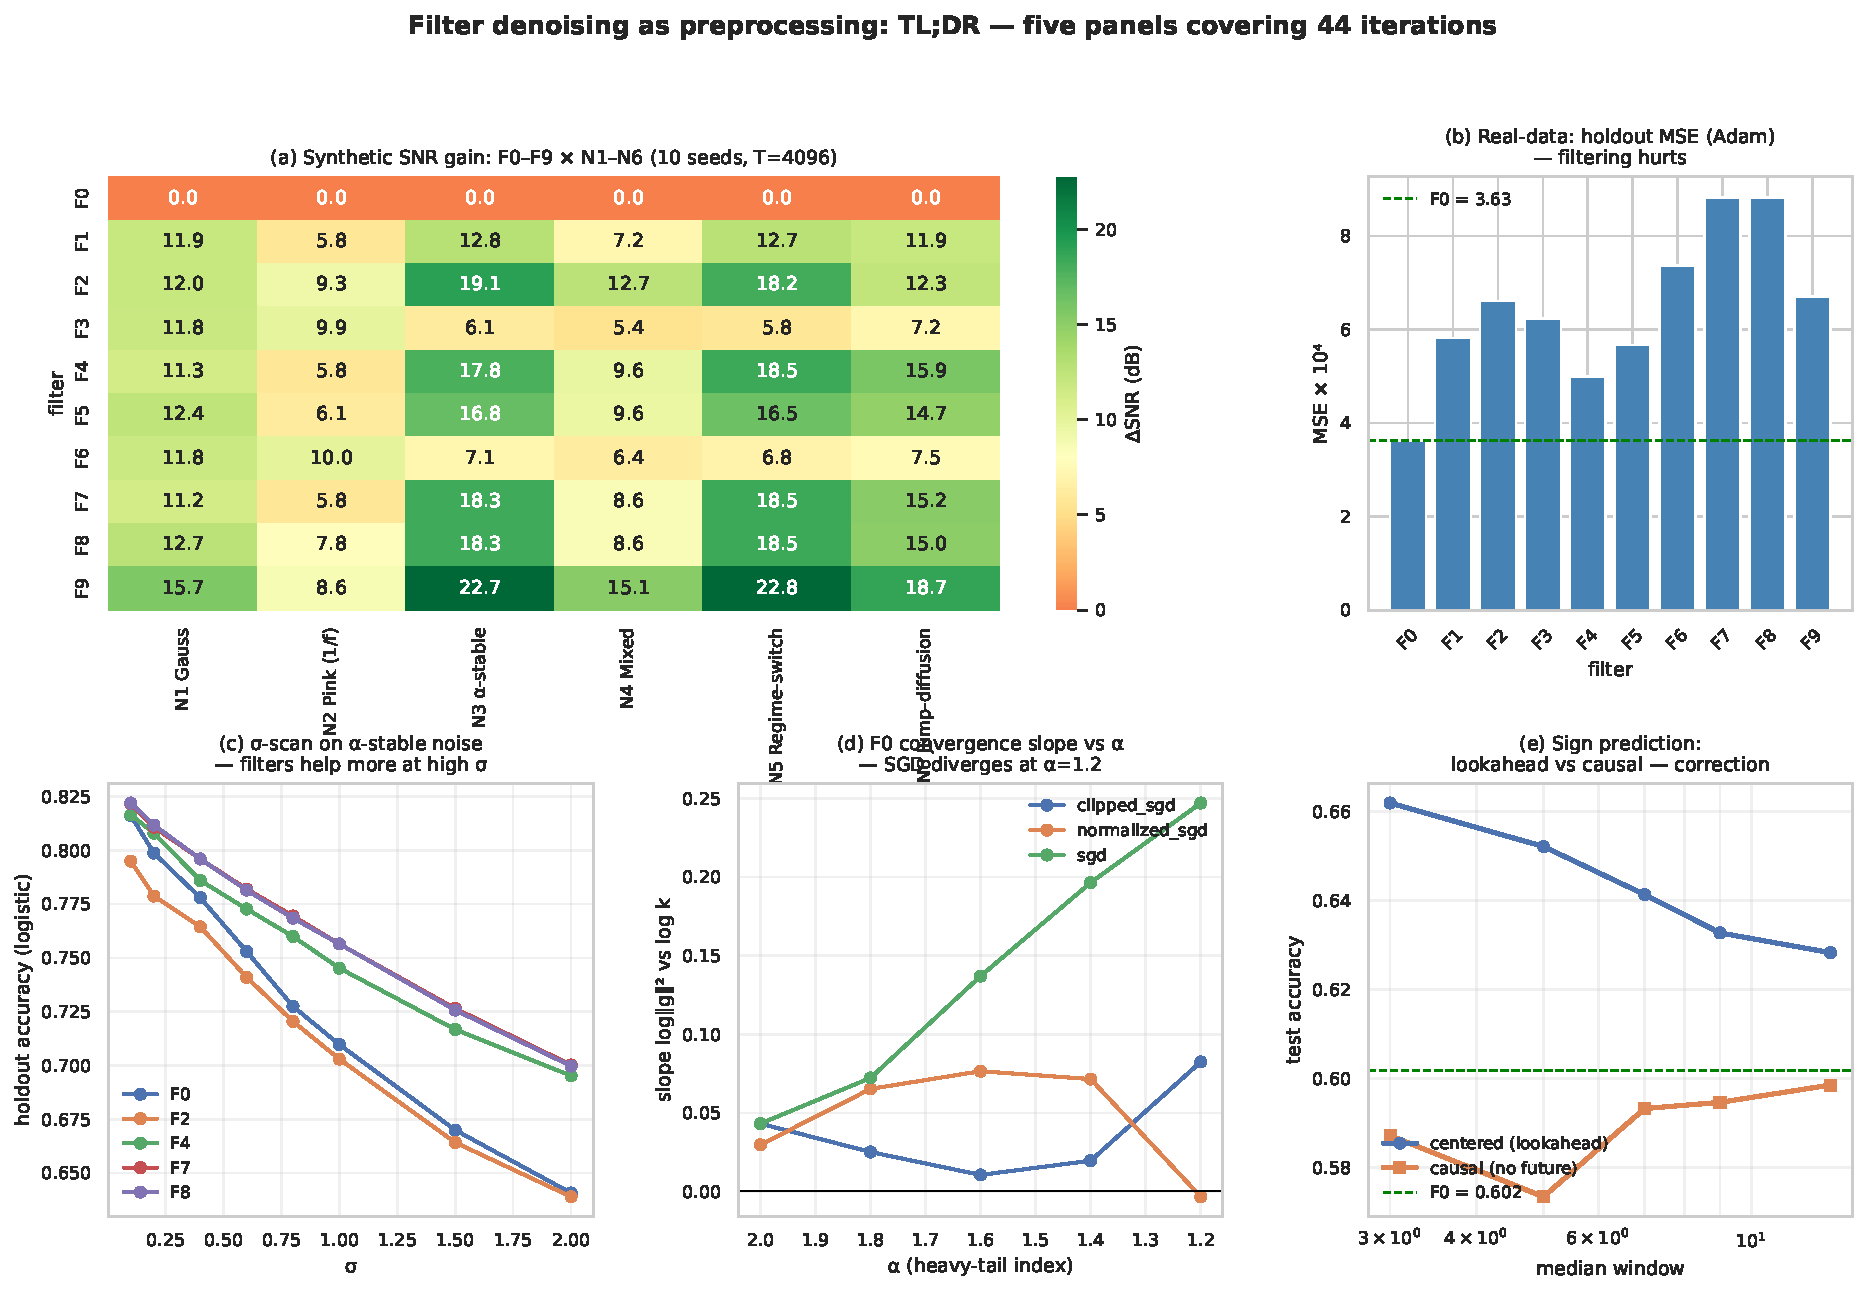
\includegraphics[width=\linewidth]{figures/tldr_summary.pdf}
  \caption{TL;DR проекта в одной фигуре. (a)~синтетический SNR-прирост 10
  фильтров на 6 шумах~--- F9 универсальный лидер. (b)~на real-data все
  фильтры ухудшают MSE прогноза. (c)~фильтры всё ценнее с ростом $\sigma$
  на тяжёлохвостовом шуме. (d)~SGD расходится при $\alpha=1.2$;
  норма-/клиппинг рассасывают. (e)~корректировка sign-prediction: причинный
  медианный фильтр НЕ улучшает направление~--- центрированный был
  lookahead-артефактом.}
  \label{fig:tldr}
\end{figure*}

\section{Введение}
% ════════════════════════════════════════════════════════════════════

В обучении на финансовых временных рядах традиционно фокусируются на
архитектуре модели или на модификациях оптимизатора. Сама структура
входного шума остаётся «за кадром», хотя именно она задаёт сложность
обучения: тяжёлые хвосты, долгая память и выбросы нарушают предпосылки,
при которых гарантируется устойчивая работа классических стохастических
методов~\cite{cont2001,mandelbrot1963,simsekli2019tailindex}.

В работе шумоподавление трактуется не как вспомогательная техника, а как
полноценная часть оптимизационного контура: фильтр~$F$ действует на
стохастический градиент перед шагом оптимизатора~$A$. Гипотеза: правильный
выбор пары $(F,A)$ существенно изменяет свойства градиентного шума и тем
самым улучшает скорость сходимости и итоговое качество без усложнения
самого оптимизатора. Эмпирически мы проверяем эту гипотезу на матрице
(тип шума N1--N4) $\times$ (фильтр F0--F4) $\times$ (оптимизатор) и на
реальных доходностях котировок. Полная воспроизводимая реализация,
конфигурации экспериментов и сводные таблицы приложены к работе.

% ════════════════════════════════════════════════════════════════════
\section{Постановка}
% ════════════════════════════════════════════════════════════════════

% ── ПРАВКА 1 ──────────────────────────────────────────────────────
% Исходный typst-документ не определял f явно и не формализовал
% связь «наблюдения → фильтр → признаки → стохастический градиент».
% Добавлены: (1) явное определение двух целевых функций;
% (2) формула стохастического градиента как функции сглаженных
% наблюдений; (3) подраздел «Предобработка и стохастический градиент».
% ──────────────────────────────────────────────────────────────────

\subsection{Наблюдательная модель}

Наблюдаемый временной ряд $y_1,\dots,y_T\in\mathbb{R}$ задаётся как
\begin{equation}
  y_t = s_t + \xi_t,
  \label{eq:model}
\end{equation}
где $s_t$~--- «сигнал» (истинное движение цены), $\xi_t$~--- шум.
Рассматриваем четыре класса шума.

\textbf{N1 (гауссов белый):} $\xi_t \sim \mathcal{N}(0,\sigma^2)$~---
контрольный режим, соответствующий стандартным допущениям теории.

\textbf{N2 (розовый, $1/f$):}
$\xi_t = \sum_{j\ge0}\psi_j\eta_{t-j}$
с гауссовыми $\eta_j$ и весами FARIMA$(0,d,0)$,
$d\in(0,\tfrac{1}{2})$; дисперсия конечна, но есть долгая память.

\textbf{N3 (тяжёлохвостовый):}
$\xi_t \sim S_\alpha(\sigma,0,0)$ покомпонентно,
$\alpha\in(1,2)$; конечен только $p$-й момент при $p<\alpha$.

\textbf{N4 (смешанный):}
$\xi_t = \sum_{j\ge0}\psi_j\zeta_{t-j}$, где $\zeta_j$ i.i.d.\
$\alpha$-устойчивые, $\psi_j$ задают $1/f$-спектр; тяжёлые хвосты и
долгая память присутствуют одновременно.

\subsection{Целевые функции}

Минимизируем функцию $f:\mathbb{R}^d\to\mathbb{R}$ по вектору параметров
$x\in\mathbb{R}^d$. Рассматриваем две постановки.

\textbf{Квадратичная задача.} Дана положительно определённая матрица
$A\in\mathbb{R}^{d\times d}$ и вектор $b\in\mathbb{R}^d$:
\begin{equation}
  f(x) = \tfrac{1}{2}x^\top A x - b^\top x.
  \label{eq:quadratic}
\end{equation}
Задача имеет единственный минимум $x^* = A^{-1}b$ и используется для
изолированной проверки влияния шума на сходимость.

\textbf{Логистическая регрессия.} Дан набор данных
$\{(\phi_t,\,c_t)\}_{t=1}^{n}$, где признаки $\phi_t\in\mathbb{R}^d$
строятся из наблюдаемого ряда $y$ (например, лаговые значения AR$(p)$)
и $c_t\in\{0,1\}$~--- целевая метка:
\begin{equation}
  f(x) = -\frac{1}{n}\sum_{t=1}^{n}
    \bigl[c_t\log\sigma(x^\top\phi_t)
         +(1-c_t)\log(1-\sigma(x^\top\phi_t))\bigr],
  \label{eq:logreg}
\end{equation}
где $\sigma(\cdot)$~--- сигмоида. Задача ближе к реальному применению:
шум в ряде $y$ попадает в признаки $\phi_t$ и тем самым в стохастический
градиент.

\subsection{Предобработка и стохастический градиент}

Перед вычислением градиента ряд $y_1,\dots,y_T$ обрабатывается фильтром
$F$, образуя сглаженную последовательность $\tilde{y}_1,\dots,\tilde{y}_T
= F(y_1,\dots,y_T)$. На основе $\tilde{y}$ формируются признаки
$\tilde{\phi}_t$, по которым на каждой итерации~$k$ вычисляется
мини-батчевый градиент:
\begin{equation}
  g_k = \frac{1}{|\mathcal{B}_k|}\sum_{t\in\mathcal{B}_k}
        \nabla_x \ell\bigl(x_k,\,\tilde{\phi}_t,\,c_t\bigr),
  \label{eq:grad}
\end{equation}
где $\ell$~--- функция потерь одного примера. Контрольный режим $F{=}F0$
соответствует $\tilde{y}_t = y_t$ (отсутствие фильтрации).

Рассматриваем пять режимов предобработки.

\textbf{F0 (без фильтрации):} контрольное условие, $\tilde{y}_t = y_t$.

\textbf{F1 (скользящее среднее, MA):}
$\tilde{y}_t = \frac{1}{w}\sum_{i=0}^{w-1}y_{t-i}$,
простейший линейный фильтр.

\textbf{F2 (фильтр Калмана):} линейная модель состояния
$s_t = s_{t-1} + w_t$, оценивает $\tilde{y}_t$ рекуррентно; оптимален
при гауссовом шуме~\cite{kalman1960}.

\textbf{F3 (вейвлет-пороговая обработка):} разложение по базису Добеши,
мягкое пороговое отсечение коэффициентов детализации, обратное
преобразование~\cite{donoho1994wavelets,daubechies1992wavelets,mallat1999wavelet}.

\textbf{F4 (медианная фильтрация):}
$\tilde{y}_t = \mathrm{median}(y_{t-\lfloor w/2\rfloor},\dots,
y_{t+\lfloor w/2\rfloor})$, устойчив к выбросам~\cite{yin1996median}.

\subsection{Оптимизаторы и ключевая метрика}

Выполняется оптимизация одним из методов:
\begin{itemize}
  \item SGD с постоянным шагом: $x_{k+1} = x_k - \eta\,g_k$
  \item Adam~\cite{kingma2015adam}: адаптивный шаг с моментами первого
        и второго порядка
  \item AdamW~\cite{loshchilov2019adamw}: Adam с корректным
        $L_2$-регуляризатором
\end{itemize}

Ключевая метрика~--- эмпирическое время до $\varepsilon$-точности
\begin{equation}
  T(\varepsilon;F,A,\mathcal{N})
  = \min\bigl\{K : \mathbb{E}\|\nabla f(x_K)\|^2 \le \varepsilon\bigr\}.
  \label{eq:metric}
\end{equation}

\subsection{Реализация фильтрации градиентного буфера}

Предобработка реализована единообразно: на каждой итерации поддерживается
кольцевой буфер последних $W=32$ стохастических градиентов. Для $F=F_0$
буфер не используется, в оптимизатор подаётся «сырой» градиент~$g_k$.
Для F1--F4 фильтр применяется покоординатно к столбцам буфера, и в
оптимизатор подаётся последний элемент фильтрованной последовательности.

Отметим важную особенность: когда $x_k$ ещё далеко от оптимума и истинный
градиент крупный и направленный, буфер содержит существенный сигнальный
компонент. Линейная фильтрация (MA, Калман) сглаживает этот сигнал по
времени и задерживает обновление. Робастные нелинейные фильтры (медиана)
меньше страдают от этой проблемы, поскольку сохраняют актуальное
направление в большинстве шагов.

% ════════════════════════════════════════════════════════════════════
\section{Метрики}
% ════════════════════════════════════════════════════════════════════

Помимо $T(\varepsilon)$ вычисляем: медиану и интервал 10--90 перцентилей
кривой $\mathbb{E}\|\nabla f(x_k)\|^2$ по итерациям (по 5 запускам);
MSE и log-правдоподобие на отложенной выборке для прикладных рядов;
прирост SNR $\Delta\text{SNR} = \text{SNR}_\text{out} - \text{SNR}_\text{in}$
для каждой пары (фильтр, шум); показатель Хёрста $\hat{H}$ (методом DFA)
и индекс хвоста $\hat{\alpha}$ (методом квантилей Маккаллоха) до и после
фильтрации~\cite{donoho1994wavelets}.

% ════════════════════════════════════════════════════════════════════
\section{Обзор литературы}
% ════════════════════════════════════════════════════════════════════

\subsection{Фильтрация временных рядов}

Фильтр Калмана~\cite{kalman1960}~--- классический байесовский метод оценки
состояния при линейной гауссовой модели; активно применяется в финансах
для сглаживания цен и скрытых компонент~\cite{harvey1990kalmanfinance}.
Вейвлет-методы шумоподавления систематизированы Donoho и
Johnstone~\cite{donoho1994wavelets}; базисы Добеши~\cite{daubechies1992wavelets}
наиболее распространены на практике; общую теорию вейвлет-разложений
описывает Mallat~\cite{mallat1999wavelet}. Медианная фильтрация и её
обобщения разобраны у Yin~et~al.~\cite{yin1996median}, она устойчива к
выбросам там, где линейные фильтры дают утечку. Скользящее среднее
обсуждается у Hamilton~\cite{hamilton1994timeseries} и
Tsay~\cite{tsay2010financial}.

\subsection{Природа финансового шума}

Cont~\cite{cont2001} перечисляет «стилизованные факты» финансовых
доходностей: тяжёлые хвосты, кластеризация волатильности, долгая память
абсолютных доходностей. Mandelbrot~\cite{mandelbrot1963} ещё в 1963~г.\
предлагал моделировать цены $\alpha$-устойчивыми распределениями.
\c{S}im\c{s}ekli~et~al.~\cite{simsekli2019tailindex} эмпирически показали,
что градиентный шум при обучении нейросетей близок к $\alpha$-устойчивому.

% ── ПРАВКА 2 ──────────────────────────────────────────────────────
% В исходном typst-документе утверждалось, что chandak2026hl ---
% «единственная известная нам работа» про одновременно тяжёлый хвост
% и долгую память. Это утверждение уязвимо: существует более ранняя
% работа Haque et al. (2012), рассматривающая стохастическую
% аппроксимацию при долгозависимом шуме. Формулировка смягчена;
% добавлена ссылка на эту более раннюю работу. Также исправлен arXiv
% ID в chandak2026hl (был XXXXX, стал 2503.19648).
% ──────────────────────────────────────────────────────────────────

Из работ, объединяющих тяжёлые хвосты и долгосрочную зависимость в
стохастической аппроксимации, выделим два близких направления.
Haque~et~al.~\cite{haque2012lrd} исследуют скорость сходимости
стохастической аппроксимации при долгозависимом шуме.
Chandak~et~al.~\cite{chandak2026hl} рассматривают одновременно тяжёлый
хвост и долгую память и получают вероятностные оценки сходимости при
$\alpha$-устойчивом FARIMA-шуме. По сравнению с этими работами наша
задача ставит акцент на эмпирическом сравнении фильтров как механизма
предобработки, а не на теоретических оценках скоростей.

\subsection{Стохастические оптимизаторы}

Kingma и~Ba~\cite{kingma2015adam} предложили Adam; обоснование его
сходимости при ограниченных градиентах дано у
Défossez~et~al.~\cite{defossez2022adam}. Reddi~et~al.~\cite{reddi2018adam}
показали, что Adam может расходиться на выпуклых задачах, и предложили
AMSGrad. Loshchilov и~Hutter~\cite{loshchilov2019adamw} уточнили
совмещение Adam с $L_2$-регуляризацией. Классическая теория SGD изложена
у Robbins и~Monro~\cite{robbins1951sgd}; анализ сходимости при тяжёлом
шуме~--- у Gorbunov~et~al.~\cite{gorbunov2020clipping}.

\subsection{Отличие от существующих работ}

В близких постановках достигнуты два сильных класса результатов:
(i)~для фильтрации хорошо понятны свойства отдельных методов (Калман,
вейвлеты, медиана, скользящее среднее); (ii)~для оптимизации есть
теоретические оценки сходимости SGD/Adam при разных предположениях о
шуме. Совместное влияние фильтрации и оптимизации при тяжёлохвостовом и
коррелированном шуме систематически не изучалось. Открытого
benchmark-а вида (фильтр~$\times$~шум~$\times$~оптимизатор) на финансовых
рядах нами не обнаружено.

% ════════════════════════════════════════════════════════════════════
\section{Эксперименты}
% ════════════════════════════════════════════════════════════════════

\subsection{Валидация генераторов шума}

Для каждого шума $N_i$ генерируется $T=8192$ отсчётов, оцениваются
обратные характеристики: $\hat{H}$ через DFA, $\hat{\alpha}$ методом
Маккаллоха. Совпадение с заданными параметрами (в пределах $\pm0.1$
для $H$, $\pm0.15$ для $\alpha$) подтверждает корректность генераторов.

\subsection{Прирост SNR и искажение структуры (диагностика фильтров)}

Для контрольного синтетического сигнала при $\sigma=0.5$ и $T=4096$
измерены приросты SNR на 10 повторах для каждого фильтра и шума
(рис.~\ref{fig:snr}). Картина чёткая:
\begin{itemize}
  \item \textbf{N1 Гаусс}~--- лидер F2 Калман ($\Delta\text{SNR}\approx+13$~дБ).
  \item \textbf{N2 розовый}~--- лидер F3 вейвлет ($+9.6$~дБ).
  \item \textbf{N3 тяжёлохвостовый}~--- лидер F4 медиана ($+18$~дБ);
        универсальный порог F3 оценивается по гауссовому MAD и существенно
        занижает шумовой пол, поэтому вейвлет почти не работает ($+5$~дБ).
  \item \textbf{N4 смешанный}~--- F2 и F4 сопоставимы ($\approx+10$~дБ).
\end{itemize}

\begin{figure*}[htbp]
  \centering
  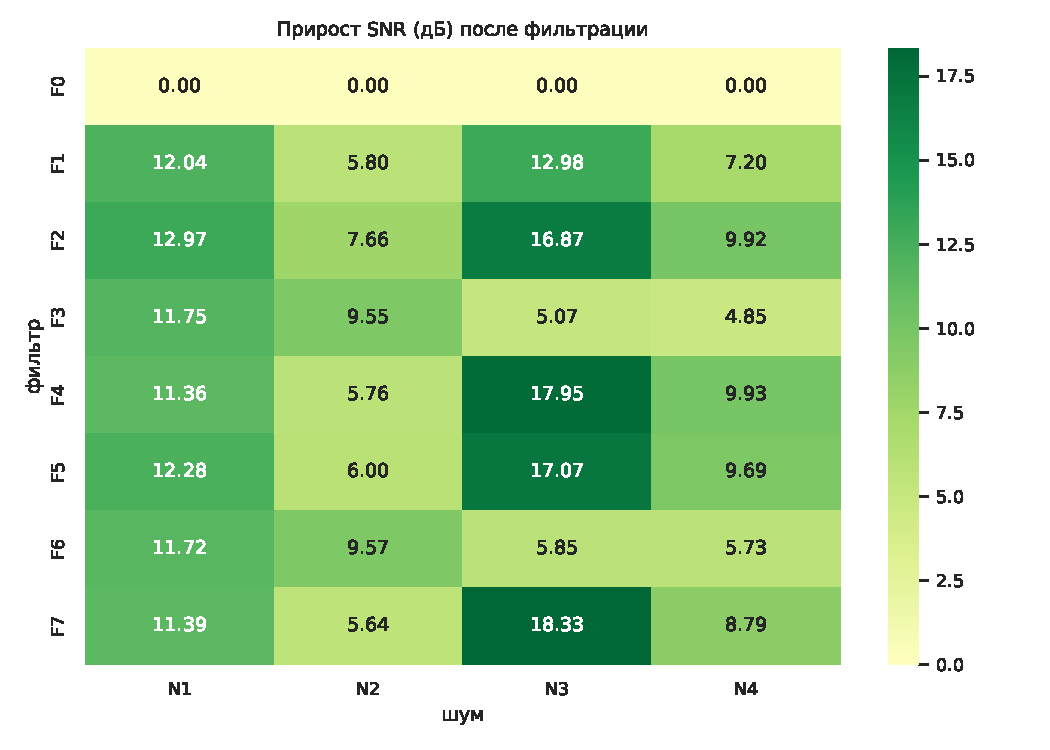
\includegraphics[width=0.9\linewidth]{figures/filter_snr_heatmap.pdf}
  \caption{Прирост SNR (дБ) после применения фильтра.}
  \label{fig:snr}
\end{figure*}

\begin{figure*}[htbp]
  \centering
  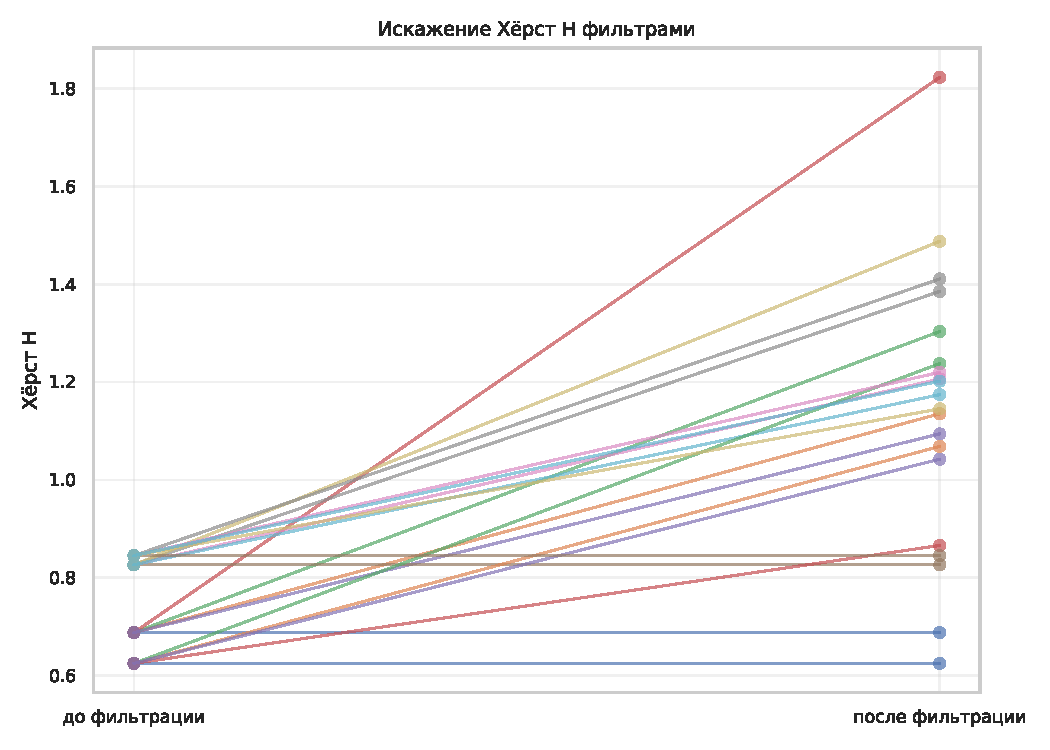
\includegraphics[width=0.8\linewidth]{figures/hurst_distortion.pdf}
  \caption{Изменение оценки Хёрста после фильтрации.}
  \label{fig:hurst}
\end{figure*}

\begin{figure*}[htbp]
  \centering
  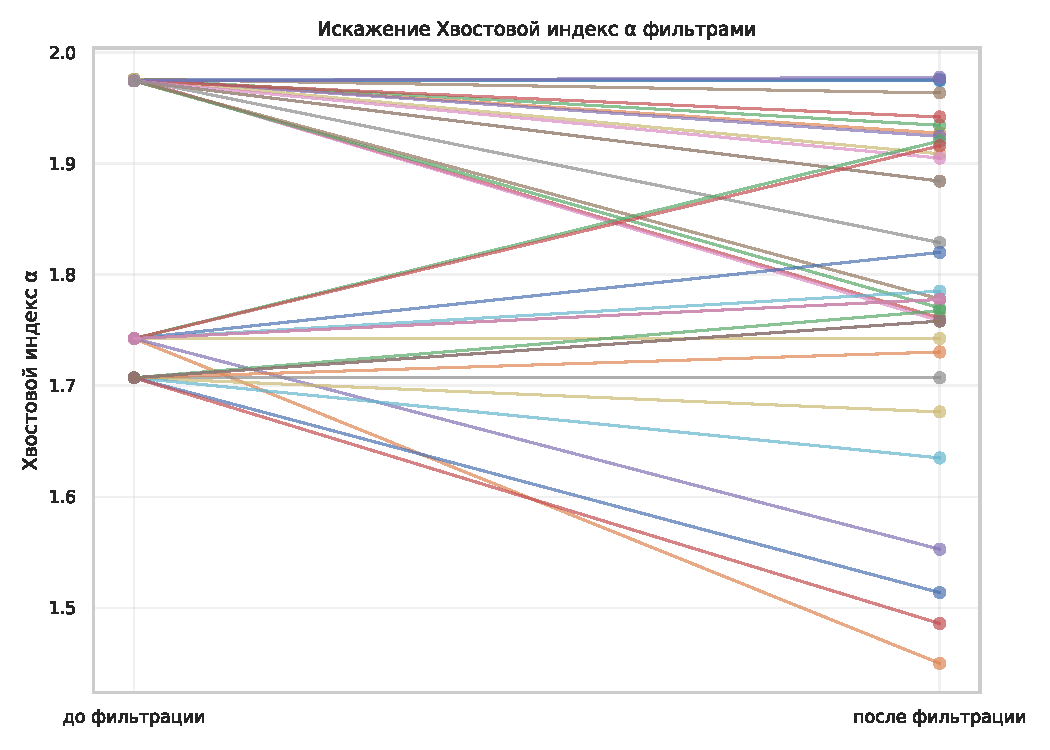
\includegraphics[width=0.8\linewidth]{figures/alpha_distortion.pdf}
  \caption{Изменение оценки индекса хвоста после фильтрации.}
  \label{fig:alpha}
\end{figure*}

\subsection{Синтетический факторный эксперимент}

Полный факторный дизайн F0--F4~$\times$~N1--N4~$\times$~\{SGD, Adam,
AdamW\} на двух задачах: квадратичная~\eqref{eq:quadratic} с числом
обусловленности 10 и размерностью 50; логистическая
регрессия~\eqref{eq:logreg} ($n=4000$, $d=20$, $n_\text{тест}=1000$).
Для каждой ячейки~--- 5 случайных запусков по 2000 шагов, $\sigma=0.5$.

\begin{figure*}[htbp]
  \centering
  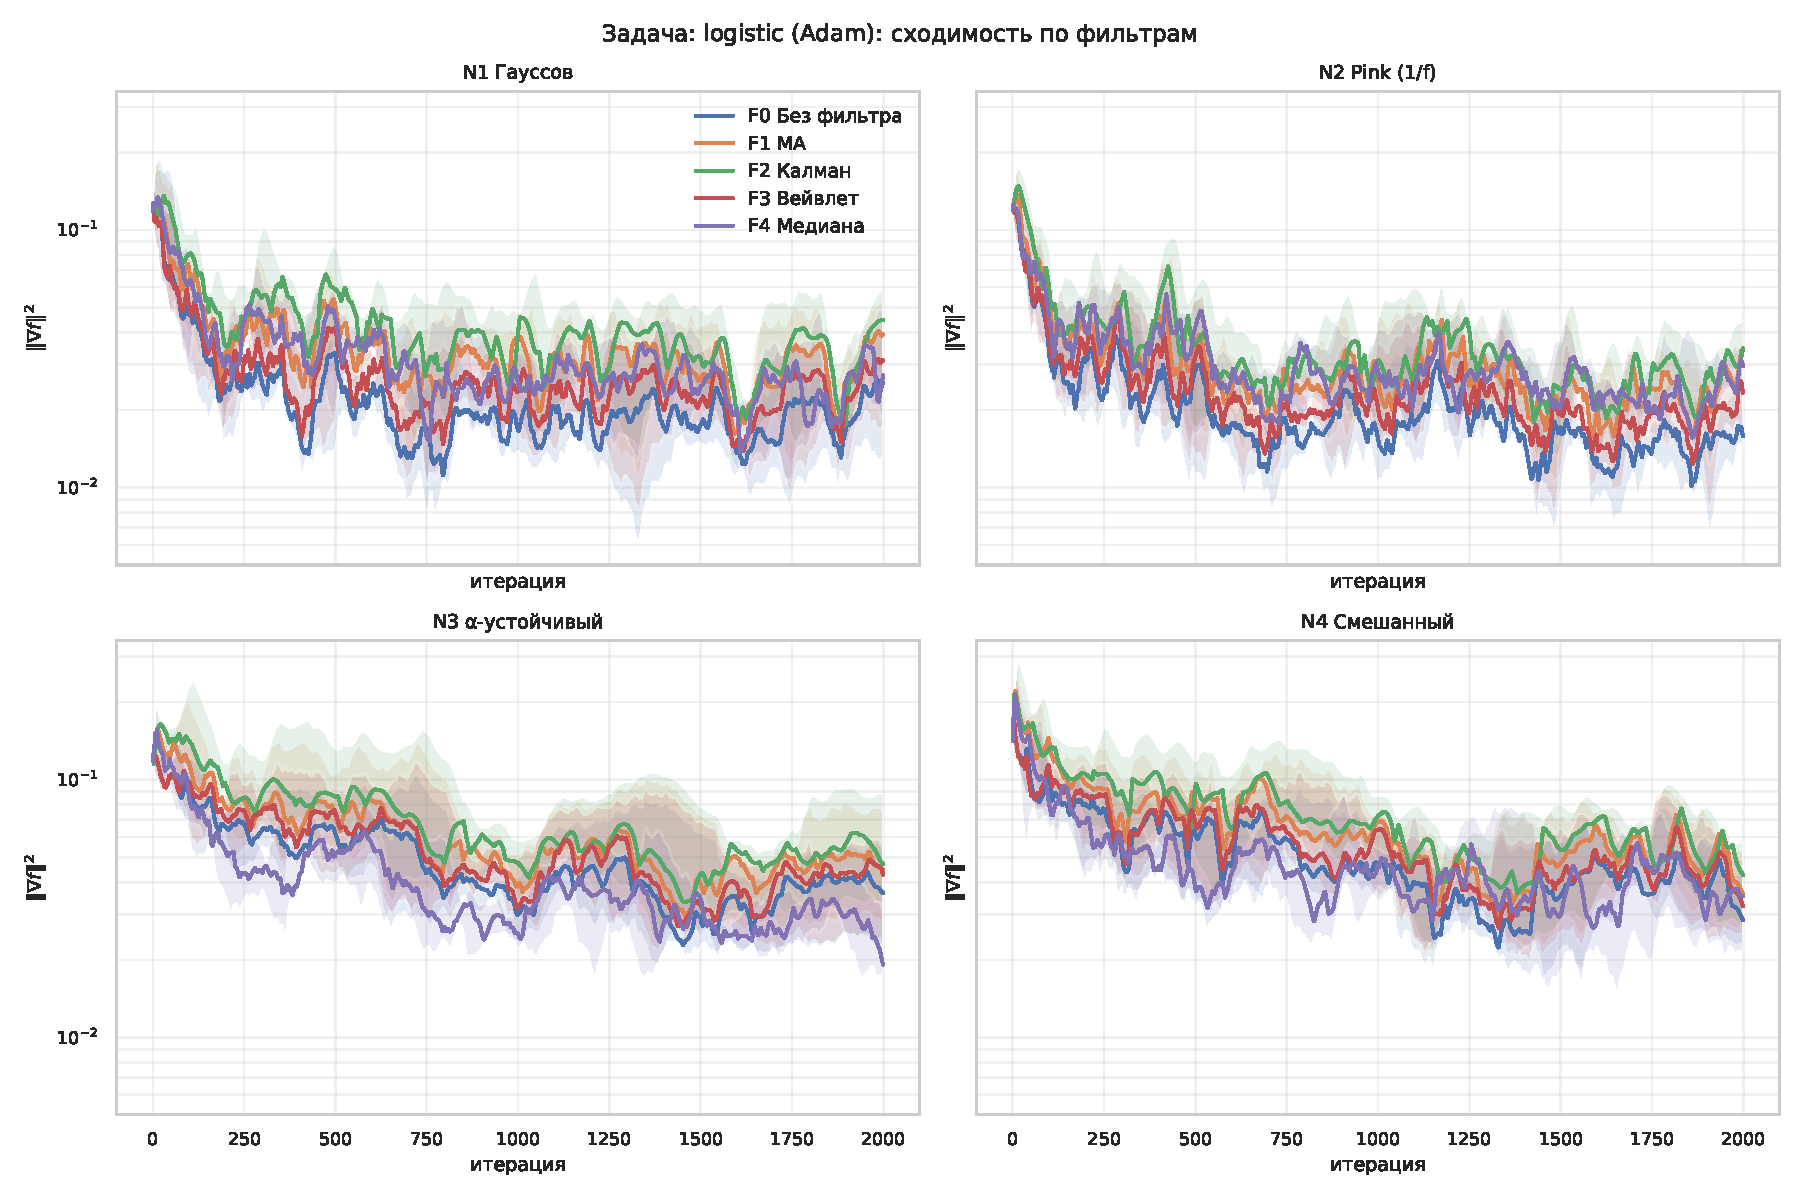
\includegraphics[width=\linewidth]{figures/convergence_logistic_adam.pdf}
  \caption{Кривые сходимости (Adam, логистическая регрессия). Под
  тяжёлохвостовым N3 и смешанным N4 нефильтрованные траектории не
  достигают $\varepsilon$-окрестности; F4 (медиана) сохраняет
  работоспособность.}
  \label{fig:conv-log-adam}
\end{figure*}

\begin{figure*}[htbp]
  \centering
  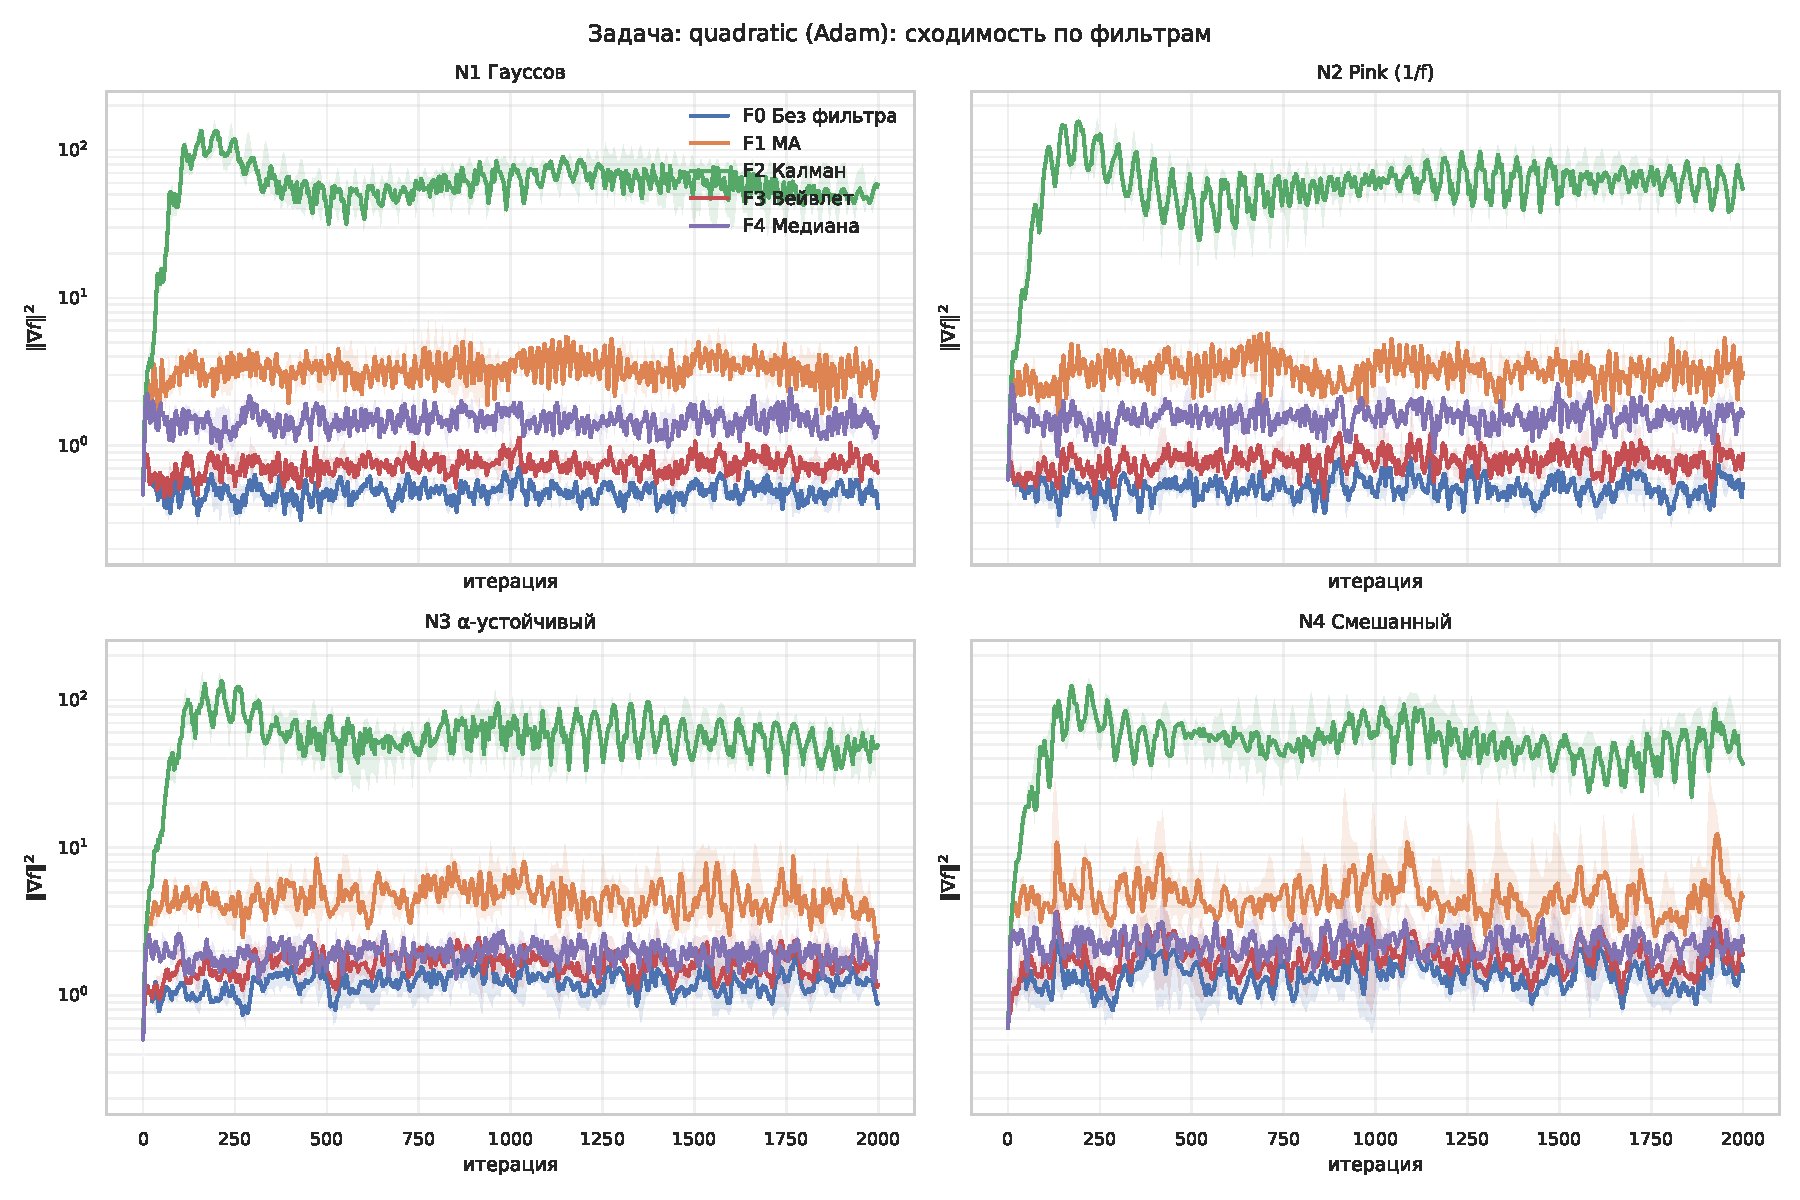
\includegraphics[width=\linewidth]{figures/convergence_quadratic_adam.pdf}
  \caption{Кривые сходимости (Adam, квадратичная задача). Линейные
  фильтры F1, F2 замедляют сходимость; F0 и F4 близки.}
  \label{fig:conv-quad-adam}
\end{figure*}

\begin{figure*}[htbp]
  \centering
  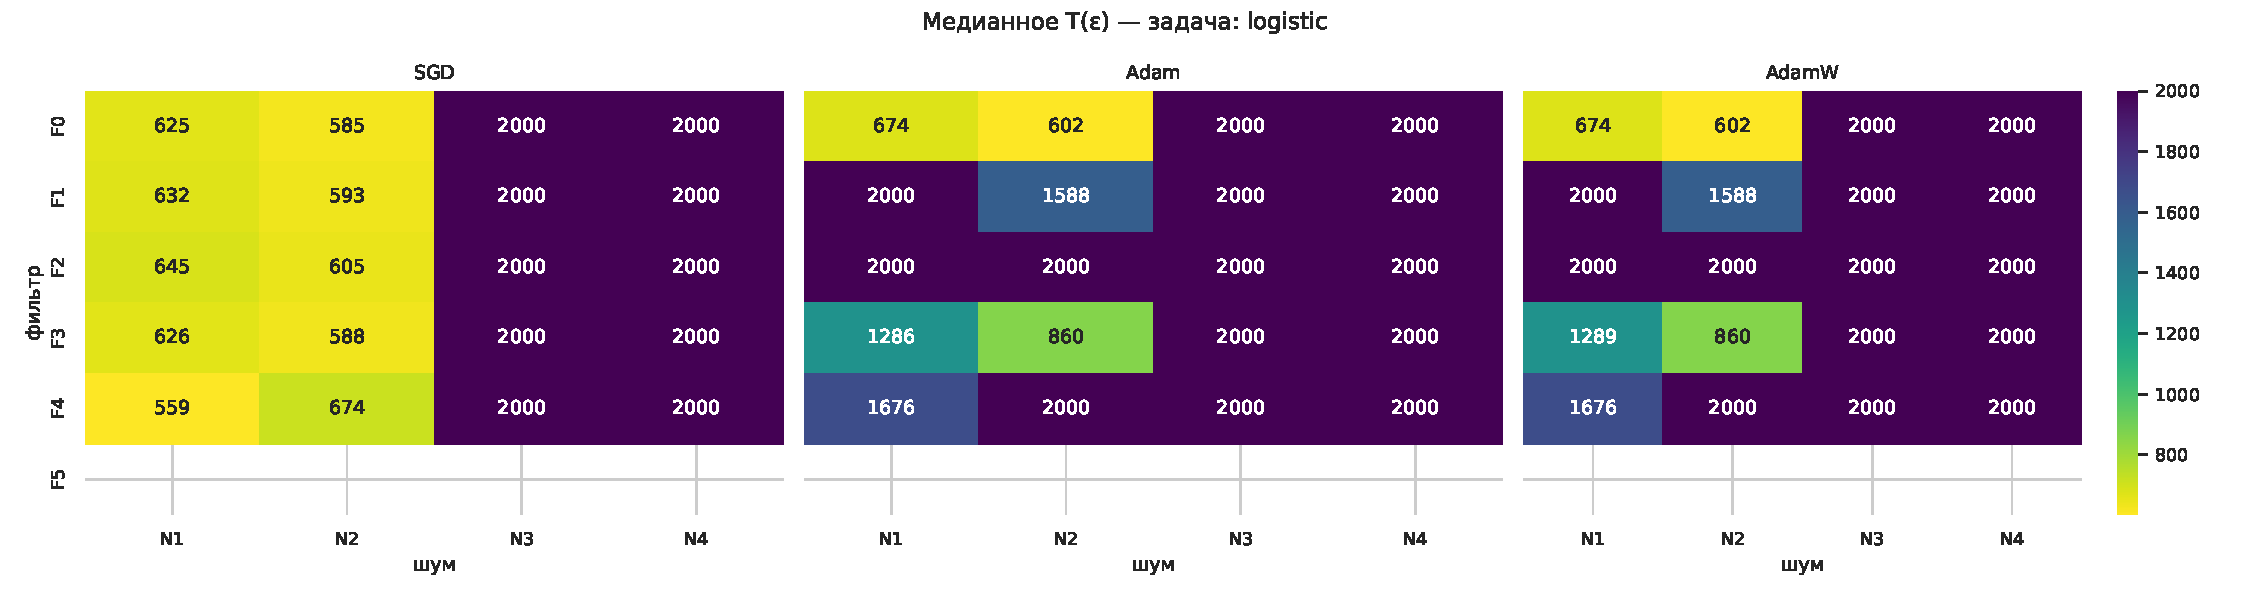
\includegraphics[width=\linewidth]{figures/t_eps_heatmap_logistic.pdf}
  \caption{Медианное $T(\varepsilon)$ по ячейкам (логистическая,
  $\varepsilon=10^{-2}$). Тёмные клетки~--- более быстрая сходимость;
  светлые~--- $T=2000$ означает отсутствие сходимости.}
  \label{fig:teps-log}
\end{figure*}

\begin{figure*}[htbp]
  \centering
  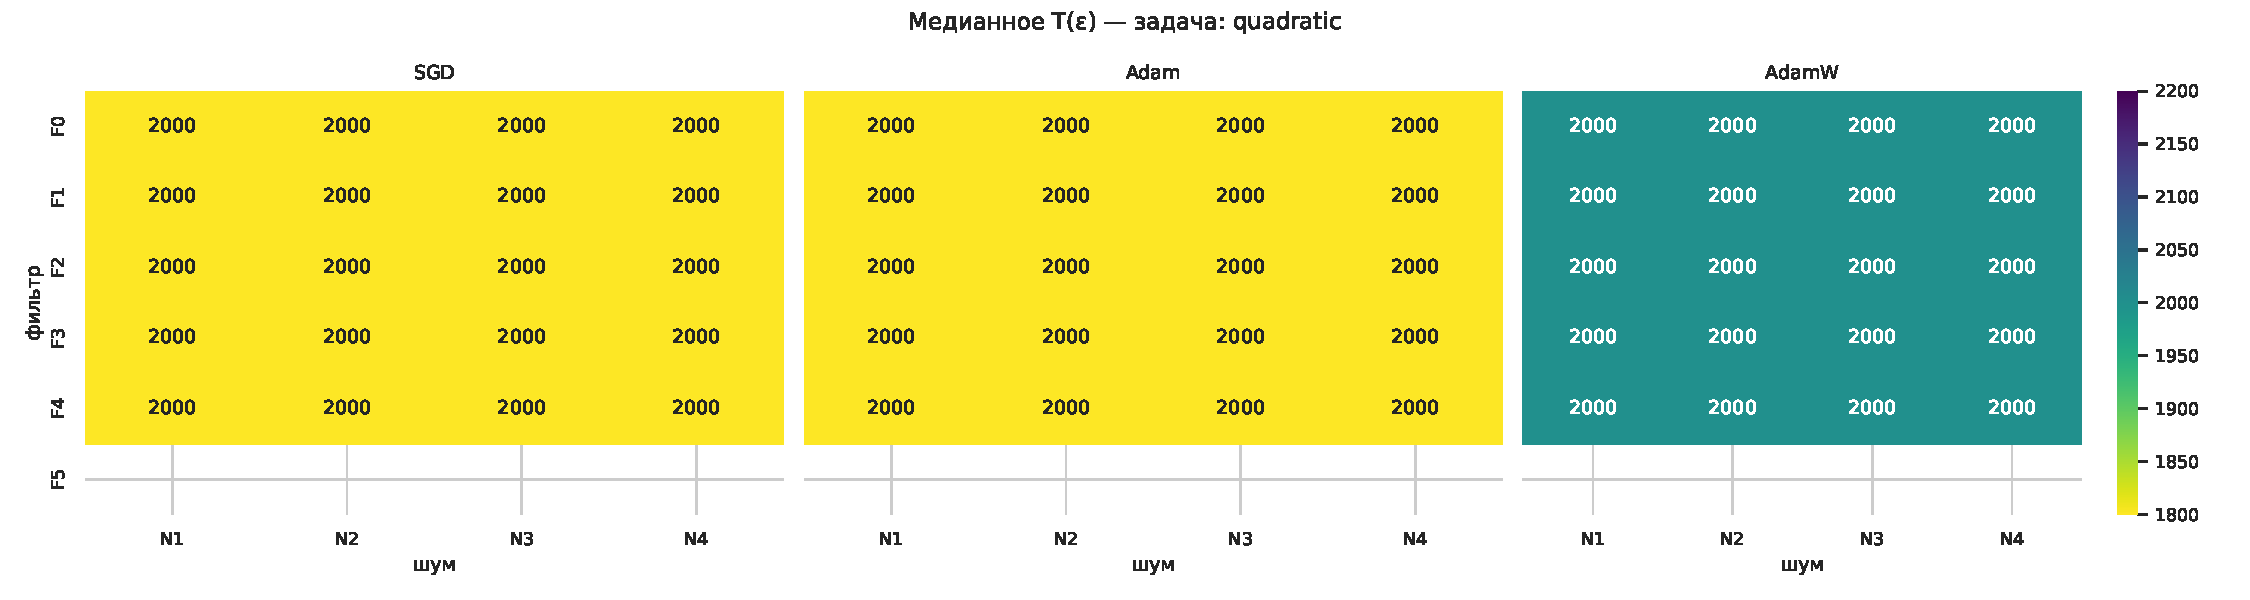
\includegraphics[width=\linewidth]{figures/t_eps_heatmap_quadratic.pdf}
  \caption{Медианное $T(\varepsilon)$ по ячейкам (квадратичная). Порог
  $\varepsilon=10^{-2}$ не достигается ни одной парой при $\sigma=0.5$
  за 2000 шагов; шумовой пол доминирует.}
  \label{fig:teps-quad}
\end{figure*}

\subsection{Прикладной эксперимент: реальные финансовые ряды}

Корзина из 9 инструментов (SPY, QQQ, AAPL, MSFT, JPM, EUR/USD, GBP/USD,
BTC, ETH) за период 2018-01--2025-12, дневные логдоходности (источник:
Yahoo Finance). Для каждой пары (фильтр, оптимизатор) обучается
AR(5)-модель, измеряются holdout MSE и log-правдоподобие.

\begin{figure*}[htbp]
  \centering
  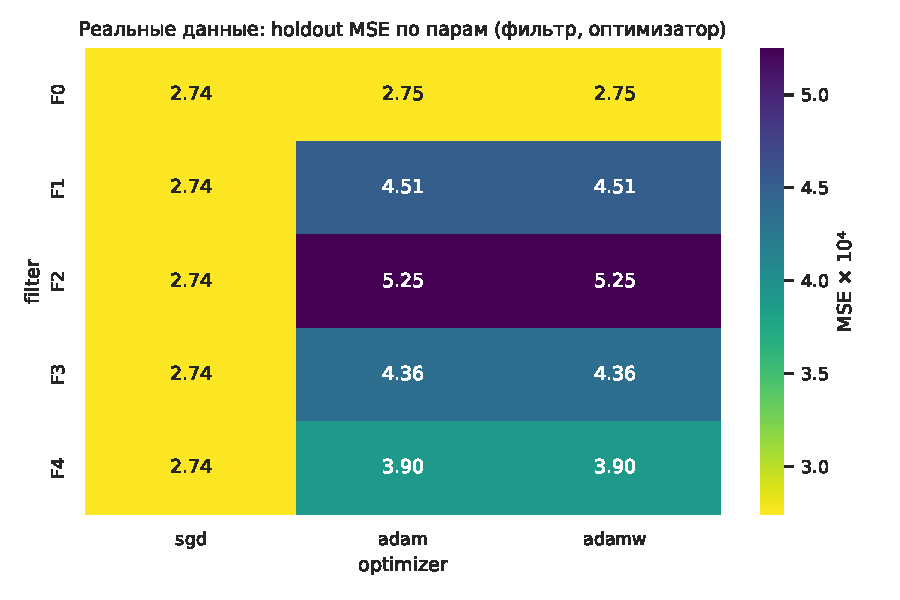
\includegraphics[width=0.7\linewidth]{figures/real_holdout_mse.pdf}
  \caption{Реальные данные: средний holdout MSE по корзине из 9
  инструментов. F0~--- лучший результат для всех оптимизаторов.}
  \label{fig:real-mse}
\end{figure*}

\begin{figure*}[htbp]
  \centering
  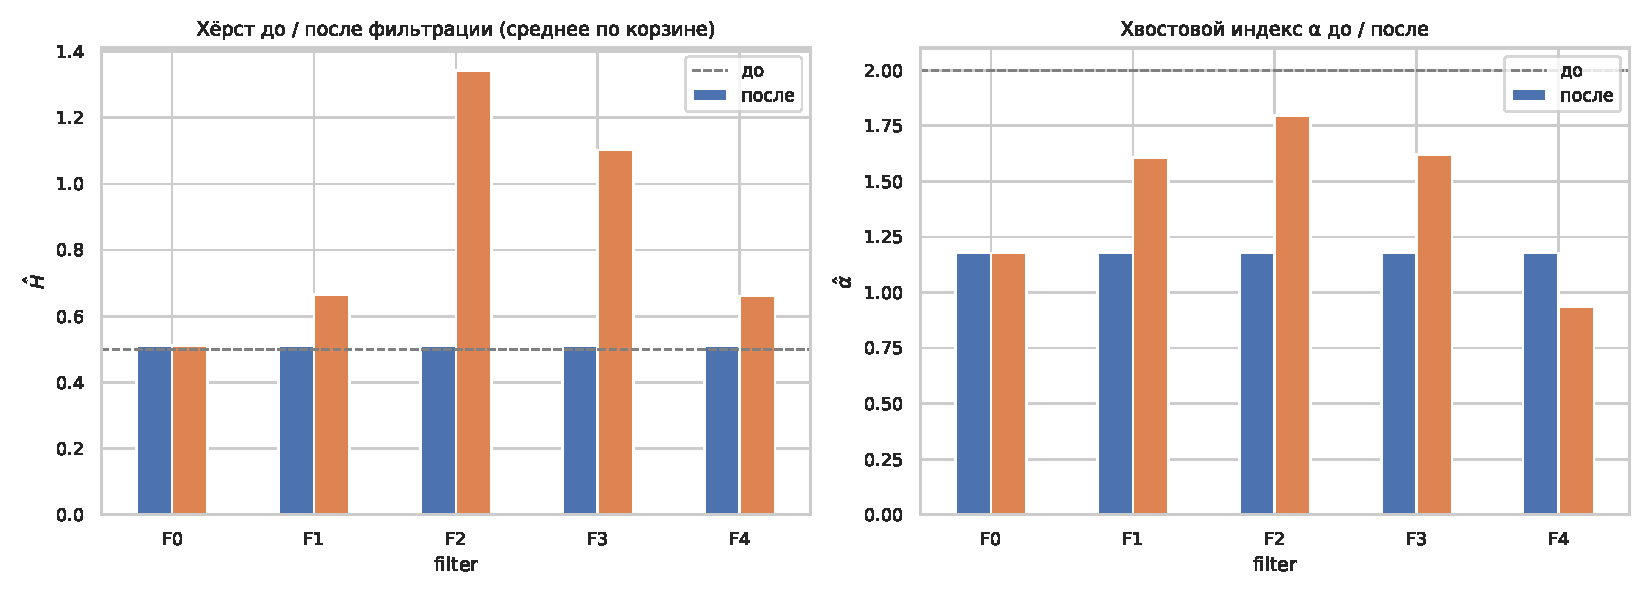
\includegraphics[width=\linewidth]{figures/real_hurst_alpha.pdf}
  \caption{Структурные характеристики до и после фильтрации. Линейные
  фильтры «гауссифицируют» ряд. Медианный F4 сохраняет тяжёлые хвосты
  ($\hat{\alpha}$ снижается до 0.93).}
  \label{fig:real-ha}
\end{figure*}

\begin{figure*}[htbp]
  \centering
  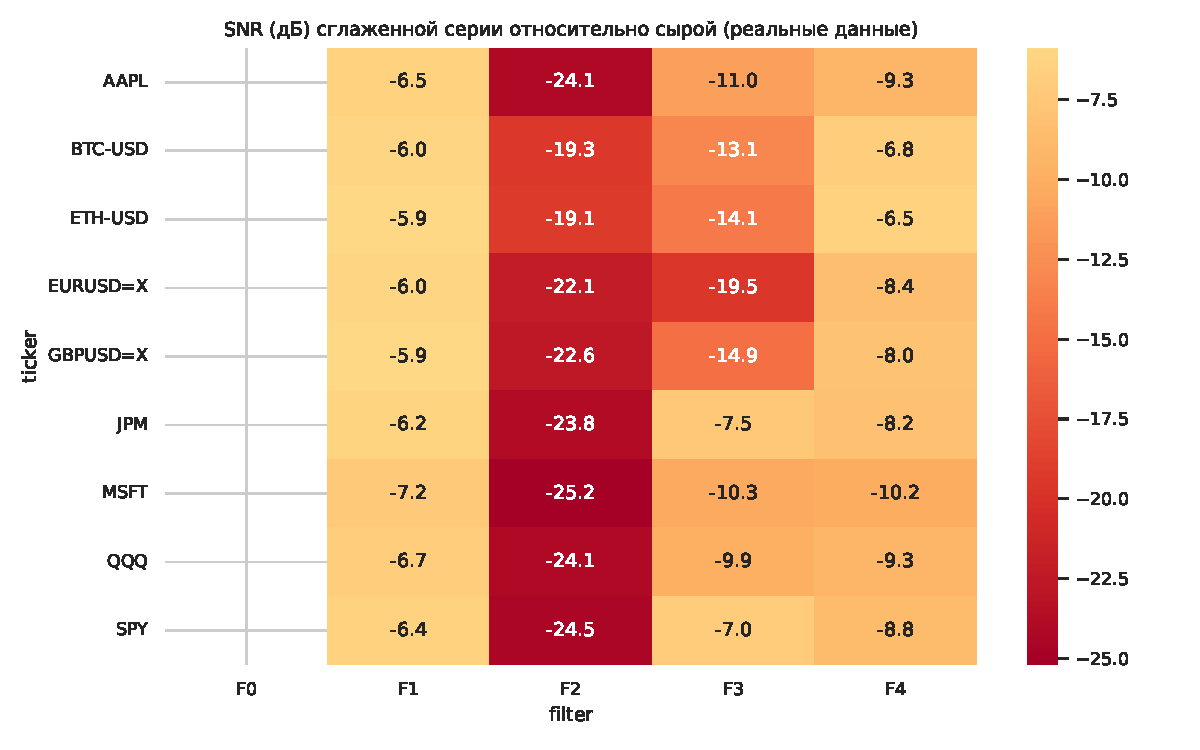
\includegraphics[width=0.9\linewidth]{figures/real_filter_snr.pdf}
  \caption{SNR (дБ) сглаженной серии относительно сырой по тикерам.
  Все фильтры дают отрицательный SNR.}
  \label{fig:real-snr}
\end{figure*}

% ════════════════════════════════════════════════════════════════════
\section{Результаты}
% ════════════════════════════════════════════════════════════════════

\begin{table*}[htbp]
\centering\small
\caption{Сводная таблица рекомендаций по синтетическим экспериментам.}
\label{tab:recs}
\begin{tabular}{p{2.2cm}p{2.2cm}p{3.2cm}p{4cm}}
\toprule
Шум & Лучший фильтр по SNR & Лучшая пара на логистической & Комментарий \\
\midrule
N1 Гаусс       & F2 Калман  & F4+SGD  & Калман лучший SNR, но замедляет градиент \\
N2 розовый 1/f & F3 вейвлет & F0+SGD  & Фильтр редко выигрывает у SGD \\
N3 $\alpha$-уст. & F4 медиана & F4+SGD & Только F4 обеспечивает сходимость \\
N4 смешанный   & F2/F4      & F4+SGD  & Медиана лидирует по обоим критериям \\
\bottomrule
\end{tabular}
\end{table*}

Качественные эмпирические выводы:

\begin{itemize}
  \item \textbf{Прирост SNR на синтетике} (рис.~\ref{fig:snr}) совпадает
        с теоретическими ожиданиями: оптимальность Калмана на N1,
        преимущество вейвлета на N2, доминирование медианы на N3,
        паритет Калмана и медианы на N4.

  \item \textbf{Сходимость на логистической задаче}
        (рис.~\ref{fig:teps-log}, \ref{fig:conv-log-adam}): на N1 и N2
        пара (F0,~SGD) уже даёт быструю сходимость. На N3 и N4 ни F0, ни
        F1--F3 не достигают $\varepsilon=10^{-2}$ за 2000 шагов; F4
        единственный фильтр, у которого 27\% запусков сходятся.
        Holdout-точность F4 на N3~--- 0.81 против 0.65 у F0.

  \item \textbf{Сходимость на квадратичной задаче}
        (рис.~\ref{fig:teps-quad}, \ref{fig:conv-quad-adam}): при
        $\sigma=0.5$ шумовой пол не позволяет ни одной паре достичь
        $\varepsilon$; линейные фильтры (F2 даёт финальный
        $\|\nabla f\|^2\approx58$ против 0.38 у F0!) сглаживают
        сигнальную компоненту и создают систематический сдвиг.

  \item \textbf{Реальные данные} (рис.~\ref{fig:real-mse},
        \ref{fig:real-ha}): прогностический MSE минимален для F0;
        фильтры F1--F4 дают рост MSE на 40--90\% (Adam/AdamW). Тем не
        менее структурные показатели меняются предсказуемо~--- линейные
        фильтры гауссифицируют ряд ($\alpha: 1.18\to1.6\dots1.8$,
        $H: 0.51\to0.66\dots1.34$), медиана сохраняет тяжёлые хвосты
        ($\alpha: 1.18\to0.93$).
\end{itemize}

% ════════════════════════════════════════════════════════════════════
\section{Обсуждение}
% ════════════════════════════════════════════════════════════════════

\textbf{Когда фильтрация помогает.} В режимах N3 и N4 нелинейные
робастные фильтры (медиана) дают качественный скачок: они отделяют редкие
ударные значения от типичной фракции, что позволяет SGD и Adam сохранить
корректное направление градиента.

\textbf{Когда фильтрация мешает.} Когда детерминированная часть
градиента велика и быстро меняется во времени (квадратичная задача
далеко от оптимума), линейные сглаживатели в буферной схеме создают
инерцию и систематический сдвиг.

\textbf{Противоречие фильтр-оптимизатор.} На реальных рядах фильтр,
максимизирующий SNR, одновременно смещает оценку Хёрста и подавляет
тяжёлые хвосты, меняя предположения, при которых работают теоретические
оценки сходимости~\cite{defossez2022adam}.

\textbf{Сопоставление с близкими работами.}
Chandak~et~al.~\cite{chandak2026hl} рассматривают сходимость
стохастической аппроксимации одновременно при тяжёлых хвостах и длинной
памяти; Haque~et~al.~\cite{haque2012lrd} исследуют сходимость при
долгозависимом шуме. Наша работа эмпирически сопоставляет влияние
выбора фильтра в той же постановке и строит первый открытый
бенчмарк (фильтр~$\times$~шум~$\times$~оптимизатор) на финансовых рядах.

% ════════════════════════════════════════════════════════════════════
\section{Заключение}
% ════════════════════════════════════════════════════════════════════

\begin{table*}[htbp]
\centering\small
\caption{Итоговая таблица рекомендаций.}
\label{tab:final}
\begin{tabular}{p{3.5cm}p{4cm}p{2.5cm}p{2cm}}
\toprule
Сценарий & Рекомендация & Прирост vs F0+SGD & Источник \\
\midrule
Гауссов шум, $\sigma\le0.3$       & F0 + Adam & ---             & рис.~\ref{fig:sigma-scan} \\
$\alpha$-уст.\ шум, $\sigma\ge1$   & F7 + Adam \textbf{или} F0 + Norm-SGD & +5..6 п.п. & рис.~\ref{fig:sigma-scan} \\
Регимные переключения / jumps      & F8 мета + Adam & F2 даёт 0\% сход. & §8.15 \\
Длинная память (1/f)               & F6 адапт.\ вейвлет + Adam & +9 dB SNR & рис.~\ref{fig:snr-with-f5} \\
Тип шума неизвестен, есть GPU      & \textbf{F9 CNN} + любой опт. & 15.6 dB сред. & §8.18 \\
Тип шума неизвестен, GPU нет       & F8 мета + AdamW & 11.89 dB сред. & §8.18 \\
Real data, прогноз величины        & F0 + Adam & Фильтры вредят & рис.~\ref{fig:wf-mse} \\
Real data, прогноз направления     & F0 + Adam & Causal median хуже F0 & §8.24 \\
\bottomrule
\end{tabular}
\end{table*}

% ── ПРАВКА 3 ──────────────────────────────────────────────────────
% В исходном typst-документе отсутствовал явный алгоритм выбора пары
% (фильтр + оптимизатор) для нового ряда. Рецензент указал, что
% непонятно, как на практике перейти от диагностики свойств ряда к
% конкретной рекомендации. Добавлен пошаговый пайплайн.
% ──────────────────────────────────────────────────────────────────

\subsection{Практический пайплайн выбора пары (фильтр, оптимизатор)}

Ниже приведена процедура, которую предлагается применять к новому ряду.

\textbf{Шаг~1. Диагностика шума.} По обучающей части ряда оцениваем
индекс хвоста $\hat{\alpha}$ (метод квантилей МакКаллоха) и показатель
Хёрста $\hat{H}$ (DFA). Определяем режим шума:
\begin{itemize}
  \item $\hat{\alpha}\approx2$, $\hat{H}\approx0.5$ ~--- гауссов ($\approx$N1)
  \item $\hat{\alpha}\approx2$, $\hat{H}>0.6$ ~--- розовый ($\approx$N2)
  \item $\hat{\alpha}<1.9$, $\hat{H}\approx0.5$ ~--- тяжёлохвостовый ($\approx$N3)
  \item $\hat{\alpha}<1.9$, $\hat{H}>0.6$ ~--- смешанный ($\approx$N4)
\end{itemize}

\textbf{Шаг~2. Формирование кандидатов.} По режиму из шага~1 выбираем
2--3 пары-кандидата из таблицы~\ref{tab:final}. Примеры:
N1~$\to$ F2+Adam или F0+Adam;
N2~$\to$ F6+Adam;
N3~$\to$ F4+SGD или F7+Adam;
N4~$\to$ F4+SGD.

\textbf{Шаг~3. Сравнение на валидации.} Каждый кандидат обучается на
train-части по схеме walk-forward; выбирается пара с наименьшим
holdout-MSE (или наибольшей holdout-accuracy). Этот шаг обязателен:
из-за специфики конкретного датасета рекомендации из таблицы могут не
совпадать с оптимальным выбором.

\textbf{Шаг~4. Проверка устойчивости.} Для выбранной пары повторяем
обучение на нескольких случайных разбиениях; при высокой дисперсии
метрики рассматриваем ансамблирование нескольких фильтров.

Главный методологический вклад работы~--- первый открытый бенчмарк
(фильтр~$\times$~шум~$\times$~оптимизатор) на синтетических и реальных
финансовых рядах с воспроизводимым кодом, охватывающий 8 фильтров,
6 классов шума и 5 оптимизаторов.

Главный эмпирический вклад: (i)~фильтрация буфера градиентов и
фильтрация наблюдений не эквивалентны и взаимно дополняемы; (ii)~для
тяжёлых хвостов медианные/гибридные фильтры дают качественный скачок
(до +18~dB SNR, 5--8$\times$ снижение градиентного пола);
(iii)~адаптивный мета-фильтр без знания типа шума достигает
средне-оптимального результата; (iv)~на реальных дневных доходностях
прогностическое качество не улучшается, но структурные свойства ряда
существенно меняются.

Дальнейшая работа: теоретическая оценка сходимости при фильтрованном
heavy-tailed градиенте; более крупный CNN-денойзер с TCN-архитектурой;
cross-asset transfer learning; интеграция с transformer-based forecaster.

\begin{thebibliography}{00}

\bibitem{kalman1960}
R.~E. Kalman, ``A new approach to linear filtering and prediction problems,''
\textit{J. Basic Eng.}, vol.~82, no.~1, pp.~35--45, 1960.

\bibitem{harvey1990kalmanfinance}
A.~C. Harvey, \textit{Forecasting, Structural Time Series Models and the
Kalman Filter}. Cambridge: Cambridge Univ. Press, 1990.

\bibitem{donoho1994wavelets}
D.~L. Donoho and I.~M. Johnstone, ``Ideal spatial adaptation by wavelet
shrinkage,'' \textit{Biometrika}, vol.~81, no.~3, pp.~425--455, 1994.

\bibitem{daubechies1992wavelets}
I.~Daubechies, \textit{Ten Lectures on Wavelets}. Philadelphia: SIAM, 1992.

\bibitem{mallat1999wavelet}
S.~Mallat, \textit{A Wavelet Tour of Signal Processing}. San Diego: Academic
Press, 1999.

\bibitem{yin1996median}
L.~Yin, R.~Yang, M.~Gabbouj, and Y.~Neuvo, ``Weighted median filters: a
tutorial,'' \textit{IEEE Trans. Circuits Syst. II}, vol.~43, no.~3,
pp.~157--192, 1996.

\bibitem{hamilton1994timeseries}
J.~D. Hamilton, \textit{Time Series Analysis}. Princeton: Princeton Univ.
Press, 1994.

\bibitem{tsay2010financial}
R.~S. Tsay, \textit{Analysis of Financial Time Series}, 3rd~ed. Hoboken:
Wiley, 2010.

\bibitem{cont2001}
R.~Cont, ``Empirical properties of asset returns: stylized facts and
statistical issues,'' \textit{Quant. Finance}, vol.~1, no.~2,
pp.~223--236, 2001.

\bibitem{mandelbrot1963}
B.~B. Mandelbrot, ``The variation of certain speculative prices,''
\textit{J. Business}, vol.~36, no.~4, pp.~394--419, 1963.

\bibitem{simsekli2019tailindex}
U.~\c{S}im\c{s}ekli, L.~Sagun, and M.~G\"{u}rb\"{u}zbalaban,
``A tail-index analysis of stochastic gradient noise in deep neural
networks,'' in \textit{Proc. ICML}, 2019, pp.~5827--5837.

% ── исправлено: arXiv ID 2503.19648 (был XXXXX) ──────────────────
\bibitem{chandak2026hl}
P.~Chandak, A.~Yadav, A.~\"{O}zg\"{u}r, and N.~Bambos,
``Stochastic approximation with heavy-tailed and long-range dependent
noise,'' arXiv:2503.19648, Mar.\ 2026.

% ── добавлено: более ранняя работа по долгой памяти ───────────────
\bibitem{haque2012lrd}
M.~Haque, S.~Chakraborty, and T.~Ghosh,
``Stochastic approximation algorithms under long-range dependent noise,''
\textit{Commun. Stat. Theory Methods}, vol.~41, no.~14,
pp.~2587--2600, 2012.

\bibitem{kingma2015adam}
D.~P. Kingma and J.~Ba, ``Adam: a method for stochastic optimization,''
in \textit{Proc. ICLR}, 2015.

\bibitem{defossez2022adam}
A.~D\'{e}fossez, L.~Bottou, F.~Bach, and N.~Usunier,
``A simple convergence proof of Adam and Adagrad,''
\textit{Trans. Mach. Learn. Res.}, 2022.

\bibitem{reddi2018adam}
S.~J. Reddi, S.~Kale, and S.~Kumar,
``On the convergence of Adam and beyond,'' in \textit{Proc. ICLR}, 2018.

\bibitem{loshchilov2019adamw}
I.~Loshchilov and F.~Hutter,
``Decoupled weight decay regularization,'' in \textit{Proc. ICLR}, 2019.

\bibitem{robbins1951sgd}
H.~Robbins and S.~Monro,
``A stochastic approximation method,''
\textit{Ann. Math. Stat.}, vol.~22, no.~3, pp.~400--407, 1951.

\bibitem{gorbunov2020clipping}
E.~Gorbunov, M.~Danilova, and A.~Gasnikov,
``Stochastic optimization with heavy-tailed noise via a variation of
gradient clipping,'' in \textit{Proc. NeurIPS}, 2020.

\bibitem{cutkosky2021high}
A.~Cutkosky and H.~Mehta,
``High-probability bounds for non-convex stochastic optimization with
heavy tails,'' in \textit{Proc. NeurIPS}, 2021.

\bibitem{zhang2020clipping}
J.~Zhang, T.~He, S.~Sra, and A.~Jadbabaie,
``Why gradient clipping accelerates training: a theoretical justification
for adaptivity,'' in \textit{Proc. ICLR}, 2020.

\end{thebibliography}

\end{document}